\documentclass[a4paper]{article}

\usepackage[spanish]{babel}
\usepackage{graphicx}

\title{ASIeR}
\author{Amalio}
\date{28 de octubre de 2022}
\begin{document}
\maketitle
\tableofcontents
\section[Idea]{Intraducción a la idea}
\paragraph{}
La idea tecnológica de este proyecto es construir una web,
que a la vez sea instalable en el móvil (PWA) con funciones de notificación,
base de datos y usando la librería de componentes de Material UI, inspirada en la filosofía
Material Design desarrollado por Google.
\paragraph{}
Aparte de esto, la idea general es construir una web/app
totalmente útil para difundir la información relevante de clase,
así como fechas de exámenes y tareas.
\section[Tecnologías]{Tecnologías a usar}
\subsection[Next Js]{NextJs(React)}
\paragraph{}
Esta web/app estará básicamente construida en\\ NextJs (12)
de Vercel, que trabaja sobre React (18)
creado y mantenido por Meta (Facebook).Este
framework nos permitirá ahorra tiempo de carga gracias a su
renderizado desde el servidor (SSR) y a su arquitectura de
una sola página (SPA) lo que dará dinamismo.
\subsection[Next-PWA]{next-pwa}
\paragraph{}
Next-Pwa es un módulo npm de javascript específico para NextJs que nos
permitirá crear la PWA de forma muy rápida, sencilla y sin mucha configuración extra.
\subsection[Web-Push]{web-push}
\paragraph{}
Este también es un módulo de javascript enfocado a manejar las notificaciones emergentes o 'push'
que envía la web al dispositivo.Gracias a este módulo, conseguiremos eso usando la api interna del
navegador, sin tener que usar ningún servicio externo.
\subsection[MongoDB]{MongoDB}
\paragraph{}
También hemos comentado que usaremos una base de datos, en este caso es MongoDB aunque
no se descartaría usar una que sea SQL como Postgres (Supabase).
\subsection[Mongoose]{Mongoose}
\paragraph{}
Otro módulo npm que sirve para manejar MongoDB con sus drivers sin tener que hacerlo
nosotros mismos y así simplificarlo todo.
\subsection[MUI]{Materila UI}
\paragraph{}
Esta librería de interfaces de usuario para React,\\ basada en la idea del Material Design
dará una apariencia similar a las apps de google y por tanto más familiar y conocida.
\section[Explicación de funciones]{Explicación de funciones}
\subsection[Calendario]{Calendario con alertas}
\paragraph{}
Para el calendario, tendrá en las fechas que haya examen, un icono arriba a la derecha
y si hay una tarea habrá otro icono distinto para las tareas. Aparte, al clicar en la fecha
nos listará las tareas y examenes que hubiera. Aparte, si para el examen quedan menos de dos
días, esa fecha saldrá en el calendario con un fondo rojo y en el caso de que quede menos de
un día para una tarea su fondo será naranja.
\subsection[Tareas]{Tareas}
\paragraph{}
Las tareas irán con una descripción corta y un título, aparte indicando la asignatura a la
que pertenecen y la fecha límite.

\subparagraph{}
Aparte, a la hora de visualizar las tareas, se podrán añadir comentarios, que irán listados
con el nombre del comentarista y el comentario como tal.
\paragraph{Función Adicional}
También las tareas podrían tener un botón para indicar que se ha hecho y así ver
el número de personas que las ha hecho, a modo de presión social para hacerla.

\subsection[Notificaciones]{Notificaciones}
\paragraph{}
Las notificaciones llegarán con unas vibraciones más continudas si es fecha de examen y más cortas si
es una tarea. Aparte, dentro de la notificación se indicará en el título si es tarea o exámen y
en el cuerpo o mensaje de la notificación se indicará cuando es dicha tarea o dicho exámen.

\subsection[Administradores]{Administradores}
\paragraph{}
Para los administradores habrá una página especial donde podrán mandar notificaciones o añadir 
tareas y exámenes a la app. Aparte, cada vez que añadan una tarea o un exámen se mandará una 
notificación a todos los subscritos.

\subsection[Generales]{Funciones generales}
\paragraph{borrado dinámico}
De las tareas y exámenes que ya han pasado, así no se llena la base de datos de 
archivos innecesarios.

\paragraph{reminder}
Añadir una notificación automática cuando quede menos de dos días para un examen o un día para
una tarea.

\paragraph{autenticación}
Para la autenticación general usaremos la base de datos de MongoDB, donde los usarios tendrán un nombre 
y una contraseña específica con ese nombre.También, podría considerar usar Auth0, una librería específica
para ello.\\ Aparte, el nombre se guardará en el almacenamiento local para no tener que llamar todo el rato
a la base da datos y así evitar consumir recursos.
\subparagraph{}
Una vez 'registrados', habrá un renderizado condicional, es decir, la página de inicio de sesión o registro 
solo se mostrará mientras no haya almacenado en memoria un nombre, en cuanto inicien sesión no volverá a 
aparecerles el login.

\paragraph{auth admins}
Para los administradores, debo usar un método disntinto de autenticación, ya que sus credenciales si 
deben ser 100\% secretas, por eso para ellos puede que si use Auth0 o les deje crear sus propios usuarios 
y contraseñas, pero siempre será un registro controlado por mi.Una idea sería crear una colección distinta
solo para ellos y crear una forma de añadirlos rápidamente con un simple form de dos inputs de tipo password. 
Entonces ellos (en mi presencia) irán añadiendo su usuario y contraseña de administrador enviandolo a la base 
de datos y una vez eso, ya estaría añadida dicha información, con una contraseña 
y usuario que solo ellos saben. 

\paragraph{Pupurrí de secciones }
Aquí dejo un listado de ideas que me parecen\\ interesantes e implementables:
\begin{itemize}
    \item Sección de asignaturas con videos explicativos (yt).
    \item Sección de 'resumenes' para cada exámen, por si alguien quiere aportar su resumen a la clase.
    \item Botón de 'estoy en Discord' para avisar cuando alguien está en el discord de la clase.
    \item Zona 'Encuestas' para votar cosas y funciones.
\end{itemize}
\date{\today}
\section[Resultado]{Resultado}
 Una vez acabado el core del proyecto, paso a explicar las funciones que finalmente tiene:
 \subsection[/]{Login}
 \paragraph{}
 He implementado una pantalla con login muy básica, con la función de solo iniciar sesión ya que 
 esta web app cuenta con usuarios 'predefinidos'.
 \paragraph{}
 Al hacer login, deben estar los dos inputs (nombre y contraseña) rellenos, aparte, la contraseña 
 debe cuadrar con la guardada en la variable de entorno, si no, da error y no autentica.
 \paragraph{}
 Una vez rellenados los inputs, al pulsar el botón este envía una petición a la api interna en la cual 
 se cumprueba que la contraseña sea válida, una vez pasado ese test, crea una cookie y autentica
 al usuario.
 \paragraph{}
 Esta autenticación es clave en toda la app ya que en caso de no estar verificado, no se podrá acceder
 a ningún recurso de la web.
 \paragraph{imagen}
 \begin{figure}[ht]
    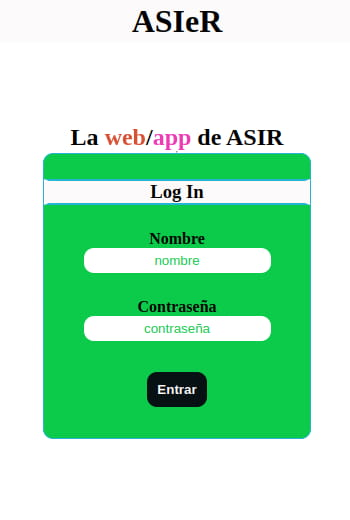
\includegraphics[scale=0.5]{./assets/login.jpg}
    \centering
    \caption{/}
    \label{fig:login}
\end{figure}
\newpage
\subsection[/app]{APP}
\paragraph{}
EN esta parte está el core de la web/app ya que es a pantalla por defecto, aquí se visualiza 
tanto el calendario, con el mes actual y el siguiente, como las tareas, exámenes y avisos.
\paragraph{calenderio}
En el calendario estarán los días, en los que si clicas te llevarán al detalle de ese día concreto.
Los días que haya exámen estarán resaltados en un rojo anaranjado, los días que haya tareas en naranja,
 los días que hay tarea y exámen en rojo fuerte con un 'x2' en un lateral, y los días que hay aviso habrá 
 un . negro a la derecha del número que indica el día.
\paragraph{exámenes}
Debajo de este calendario, está un listado con exámenes, así como tareas y otros avisos, todos 
listados en orden de fecha ascendente. Si clicas en cualquiera de ellos te llevarán al detalle, donde 
podrás agregar comentarios.
\paragraph{imagen}
\begin{figure}[ht]
   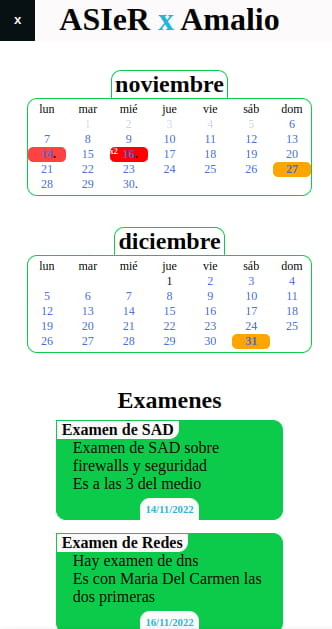
\includegraphics[scale=0.5]{./assets/app.jpg}
   \centering
   \caption{/app}
   \label{fig:app}
\end{figure}
\newpage
\subsubsection{sidebar}
\paragraph{}
El sidebar estará presente en toda la intefaz gráfica de la app y variará según el rol de usuario 
(administrador o usuario).\\ Este sidebar contiene un listado de todas las rutas disponibles para 
el usuario.
\paragraph{imagen}
\begin{figure}[ht]
   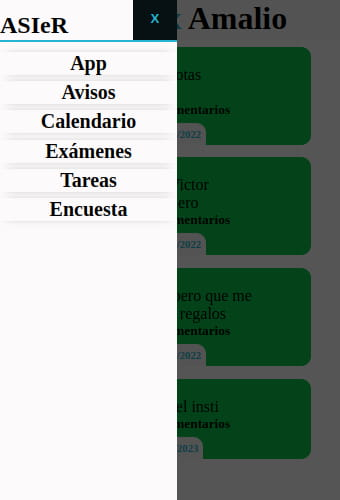
\includegraphics[scale=0.5]{./assets/sidebar.jpg}
   \centering
   \caption{sidebar}
   \label{fig:sidebar}
\end{figure}
\newpage
\subsection[/app/curso]{Curso}
\paragraph{}
Este es un subdirectorio del que cuelgan las siguientes secciones:
\subsubsection[/app/curso/avisos]{Avisos}
\paragraph{}
En esta zona se encuentran listados todos los avisos en un orden ascendiente por fecha 
(más próximos, antes). En cada aviso se muestra tanto su título, descripción y fecha como 
el número de comentarios que tiene. Pulsando en el aviso se va al detalle donde se puede comentar.
\subsubsection[/app/curso/examenes]{Exámenes}
\paragraph{}
En esta zona se encuentran listados todos los exámenes en un orden\\ ascendiente por fecha 
(más próximos, antes). En cada exámen listado se muestra tanto su título, descripción y 
fecha como el número de comentarios que tiene. Pulsando en el exámen se va al detalle 
donde se puede comentar.
\subsubsection[/app/curso/tareas]{Tareas}
\paragraph{}
En esta zona se encuentran listadas todas las tareas en un orden ascendiente\\ por fecha 
(más próximos, antes). En cada tarea se muestra tanto su título, descripción y 
fecha como el número de comentarios que tiene. Pulsando en una tarea se va al detalle 
de esta, donde se puede añadir comentarios.
\paragraph{imagen}
Al ser las tres secciones anteriores casi idénticas,  una sola imágen basta para reflejar su aspecto:
\begin{figure}[ht]
   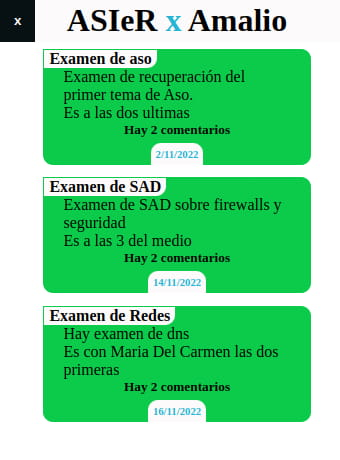
\includegraphics[scale=0.5]{./assets/examenes.jpg}
   \centering
   \caption{exámenes}
   \label{fig:examenes}
\end{figure}
\newpage
\subsubsection[/app/curso/calendario]{Calendario}
\paragraph{}
Aparte del calendario que ya viene en el /app, este es otro igual (mismas funcionalidades),
solo que con los 6 meses siguientes que preceden al actual.
\paragraph{imagen}
\begin{figure}[ht]
    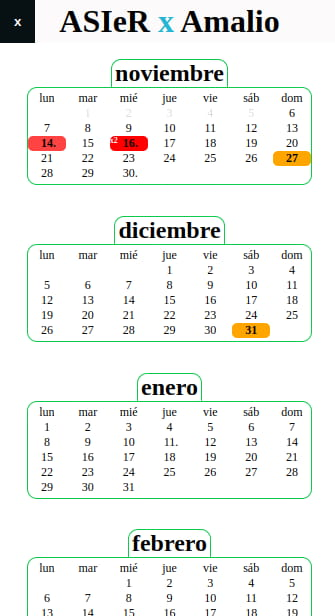
\includegraphics[scale=0.5]{./assets/calendario.jpg}
    \centering
    \caption{calendario}
    \label{fig:calendario}
 \end{figure}
 \newpage
 \subsubsection[/app/curso/encuestas]{Encuestas}
 \paragraph{}
 En esta zona están listadas las encuestas en orden descendente de adición 
 (antes añadida, más abajo) donde, al pulsar en 'votar' en alguna de ellas
 abre el detalle y se podrá votar. En cada encuesta mostrada se observa el 
 título y la descripción.
 \paragraph{imagen}
 \begin{figure}[ht]
    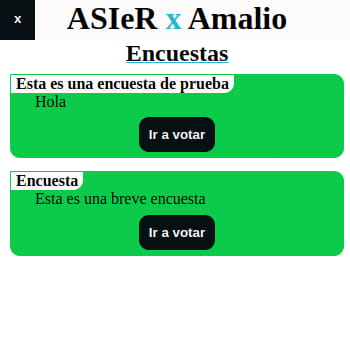
\includegraphics[scale=0.5]{./assets/encuestas.jpg}
    \centering
    \caption{encuestas}
    \label{fig:encuestas}
 \end{figure}
 \newpage
 \subsection[/app/tarea/id]{Tarea:Detalle}
 \paragraph{}
Este es el detalle de alguna tarea, exámen o aviso. En esta parte estará el título, 
la descripción, la fecha y también los comentarios así como la posibilidad de añadirlos.
\paragraph{imagen}
 \begin{figure}[ht]
    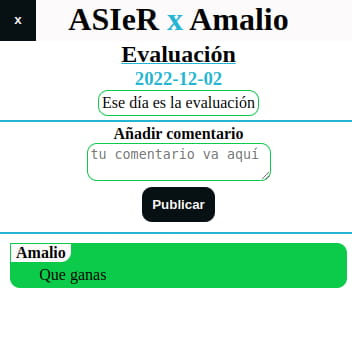
\includegraphics[scale=0.5]{./assets/tarea.jpg}
    \centering
    \caption{detalle de tarea}
    \label{fig:tarea}
 \end{figure}
 \newpage
 \subsection[/app/mes/dia]{Día:Detalle}
 \paragraph{}
 El detalle del día es muy pareceido al listado de tareas, avisos y exámenes.
 Muestar el título, descripción, número de comentarios y fecha de las tareas, exámenes o
  avisos que hay ese día. Al pulsar en alguna, lleva al detalle de la misma.
\paragraph{imagen}
 \begin{figure}[ht]
    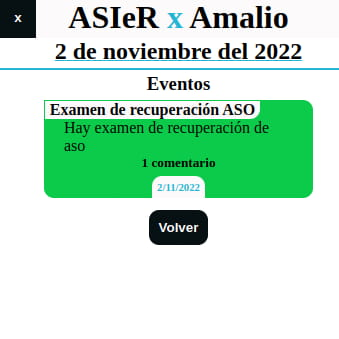
\includegraphics[scale=0.5]{./assets/monthday.jpg}
    \centering
    \caption{detalle del día}
    \label{fig:dia}
 \end{figure}
 \newpage
 \subsection[/app/admin]{Admin}
 \paragraph{}
 En esta sección se administra la adición de tareas, exámenes y avisos a la vez que 
 las notificaciones, aparte, también se añaden encuestas.\\
 Esta es una ruta protegida puesto que solo los usuarios verificados pueden acceder a ella.
 \paragraph{}
 La verificación se hace en un enlace interno que no se muestra en el sidebar.
 Este enlace, en mi caso, es el /app/control/create/one/administrator.\\
 Una vez allí, se puede crear un nuevo usuario (si esa opción está cubierta dentro 
 de las variables de entorno) o simplemente iniciar sesión.\\
 Una vez autenticado, aparecerá la sección admin dentro del sidebar:
 \begin{figure}[ht]
   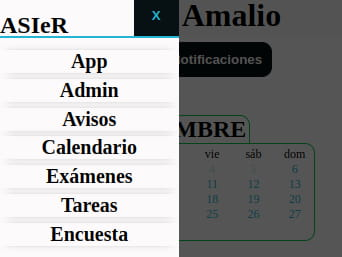
\includegraphics[scale=0.5]{./assets/admin-sidebar.jpg}
   \centering
   \caption{admin sidebar}
   \label{fig:admin-sidebar}
\end{figure}
\newpage
\paragraph{}
Dentro del admin, la interfaz en básica para realizar las acciones necesarias:
\paragraph{imagen}
 \begin{figure}[ht]
    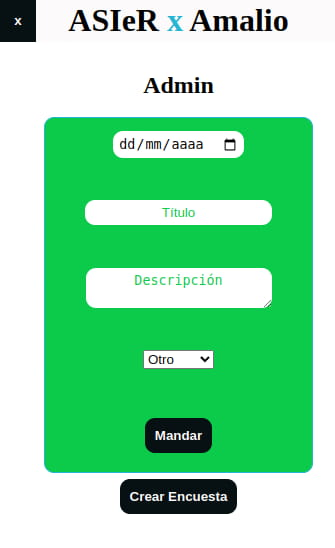
\includegraphics[scale=0.5]{./assets/admin.jpg}
    \centering
    \caption{admin}
    \label{fig:admin}
 \end{figure}
 \newpage
 \subsubsection[/app/admin/encuestas]{Admin Encuestas}
 \paragraph{}
 En esta sección, los administradores pueden crear encuestas, con tantas opciones como deseen.
 Para seleccionar x opciones, ponen el número de opciones que necesitan en el input numérico, y,
 al dar a añadir opciones, se añadirán automáticamente al cuerpo de la encuesta.
 Una vez eso, solo hace falta rellenar la encuesta con el título, descripicón y un título 
 para cada opción. Si hiciera falta explicar las opciones, se deben explicar en la descripción.
 \paragraph{imagen}
 \begin{figure}[ht]
    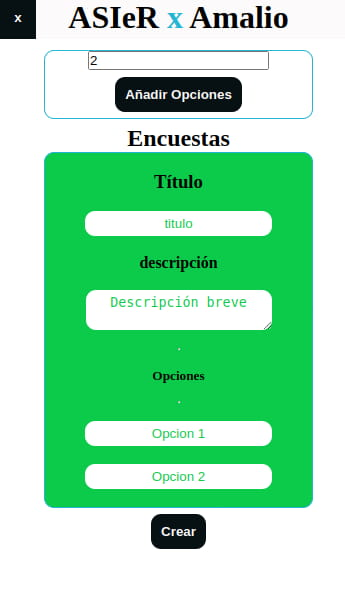
\includegraphics[scale=0.5]{./assets/add-encuesta.jpg}
    \centering
    \caption{añadir encuesta}
    \label{fig:add-encuesta}
 \end{figure}
 \newpage
 \end{document}